\documentclass[main.tex]{subfiles}

\chapter{Contextualisation}

Dans ce chapitre, nous allons définir ce qu'est un Pokémon et ce qu'est les Video Game Championship (VGC).

\section{Caractéristiques}

Les Pokémon sont des créatures fictives vivant dans la franchise éponyme qui ont des caractéristiques de par leur apparence comme les couleurs, la forme et la taille mais on retrouve aussi des traits qui influe sur leurs prises d'actions durant certains évènements tels qu'en combat ou en concours comme nous l'avons défini précédemment. Le Pokémon peut progresser au travers de l'expérience et évoluer dans un nouveau Pokémon. Dans les parties suivantes nous allons définir ce qui compose un Pokémon et ce qui peut influer ces caractéristiques.

\subsection{Propre au Pokémon}

Dans cette partie, nous allons citer les caractéristiques qui compose le Pokémon et l'influe donc directement.

\subsubsection{Le niveau du Pokémon}

Un Pokémon peut aller du niveau 1 au niveau 100. Le niveau agit sur les statistiques du Pokémon, les augmentant au fur et à mesure qu'il progresse dans son niveau. Le niveau agit aussi sur les capacités qui peuvent ne peuvent appris qu'à un certain niveau ou après.

\subsubsection{Le sexe du Pokémon}

Un Pokémon peut être male, femelle ou asexué. Le sexe peut influer sur l'évolution du Pokémon changer le Pokémon qu'il peut devenir. Certains statuts, effets ou capacités peut aussi influer le Pokémon selon son sexe.

\subsubsection{Le type du Pokémon}
\label{type_pokemon}

Dans le monde Pokémon, les Pokémon peuvent avoir des types qu'ils leur sont attribués. Un pokémon a toujours un type qui lui est associé. Depuis la seconde génération, le Pokémon peut avoir jusqu'à deux types. Voici la liste des types qui existent à l'année 2019 :

\begin{itemize}
    \item Normal
    \item Feu
    \item Eau
    \item Électrique
    \item Plante
    \item Glace
    \item Combat
    \item Poison
    \item Sol
    \item Vol
    \item Psy
    \item Insecte
    \item Pierre
    \item Spectre
    \item Dragon
    \item Ténèbres
    \item Acier
    \item Fée
\end{itemize}

Ces types ont une relation de force et de faiblesses entre elles. Un Pokémon de type feu sera plus sensible à des attaques de type eau. Une attaque de type Electrique va infliger deux fois plus de points de dégâts à un Pokémon de type Eau ou à un Pokémon de type Vol. En contrepartie, cela implique qu'il y a aussi une relation de résistance entre ces types.

Dans le cas d'une attaque de type Feu touchant un Pokémon de type Feu ou de type Eau, l'attaque n'infligera que la moitié des points de dégâts. De plus, il existe une relation dans laquelle l'attaque n'aura aucun effet sur le Pokémon, comme une attaque de type Spectre contre un Pokémon de type Normal.

Depuis la seconde génération cependant, Pokémon a vu l'introduction des Pokémon à double type. Un Pokémon de type Eau et Vol va subir, en ignorant tout les autres éléments qui influe sur les points de dégâts quatre fois plus de points de dégâts de la part d'une attaque Électrique. Dans le cas d'une attaque Électrique contre un Pokémon de type Eau et Insecte, la résistance et la faiblesse s'annule, de tel sorte que l'attaque inflige des points de dégâts sans subir les modifications des types. Dans le cas d'un type qui annule l'attaque, comme une attaque de type Spectre contre un Pokémon de type Normal, peu importe le second type du Pokémon les dégâts infligés sont nullifiés.

Vous trouverez le graphe de relation des résistances et des faiblesses entre les types dans la suite de ce chapitre à la figure 2.1.

\begin{figure}[ht]
\centering
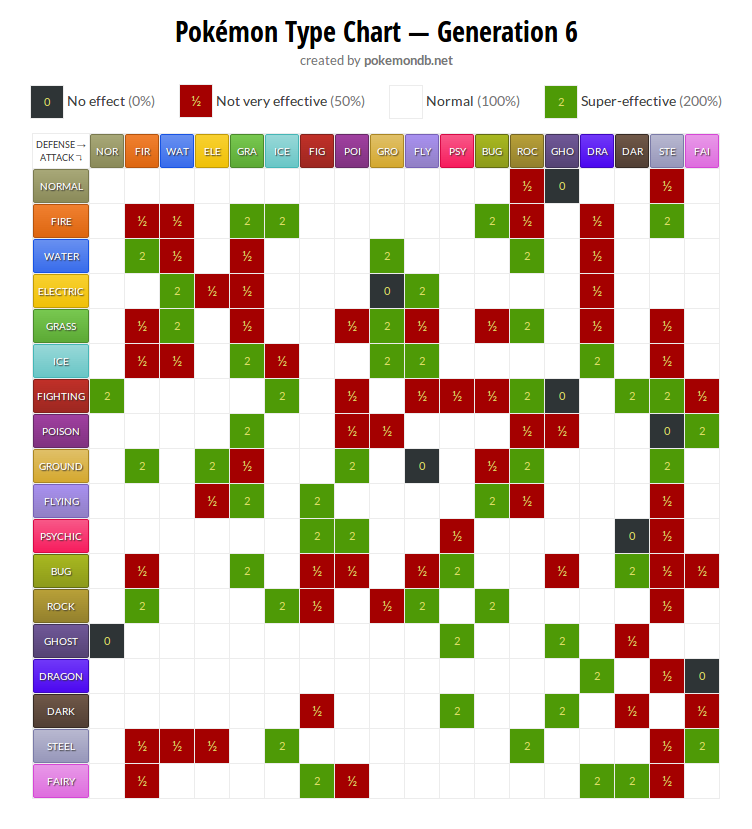
\includegraphics[width=0.85\textwidth]{img/typechart.png}
\caption{\label{fig:schema}Charte graphique des types, de leur forces et faiblesses, pokemondb.net/type}
\end{figure}

\subsubsection{Les statistiques du Pokémon}

Le Pokémon contient aussi des statistiques qui vont influencer sur ses dégâts infligés et subis et/ou sa viabilité en combat ou hors-combat. Dans cette section, nous allons décrire toutes les variables qui compose le Pokémon.

\begin{enumerate}
    \item Les points de vie
    
Un Pokémon a un nombre de point de vie maximale, qu'il ne peut pas dépasser. Si ses points de vie tombent à zéro, le Pokémon feint et n'est plus disponible pour se battre.

    \item L'Attaque
    
L'Attaque affecte les capacités physique du Pokémon. Elle intervient lors de l'affectation des points de dégâts infligés.

    \item L'Attaque Spécial
    
L'Attaque Spéciale affecte les capacités spéciale du Pokémon. Elle intervient lors de l'affectation des points de dégâts infligés.

    \item La Défense
    
La Défense affecte les capacités physique du Pokémon. Elle intervient lors de l'affectation des points de dégâts subis.

    \item La Défense Spéciale
    
La Défense Spéciale affecte les capacités spéciale du Pokémon. Elle intervient lors de l'affectation des points de dégâts subis.

    \item La Vitesse
    
La Vitesse détermine l'ordre d'action des Pokémons en combat. Sauf sous certaines exceptions, un Pokémon A dont la vitesse est supérieure à un Pokémon B attaquera en premier dans le tour.

    \item Les statistiques de base
    
Chaque Pokémon a des statistiques de base qui lui sont propres. Les statistiques notées ci-dessus peuvent fluctuer selon certains facteurs dont les statistiques de base du Pokémon concerné. Les statistiques de base ne changeront pas durant la progression du Pokémon.

    \item Les Points Individuelles - IV
    
Les points individuelles, ou IV, sont déterminées à la naissance du Pokémon ou lors de sa rencontre dans la nature. Les IV sont générées de manière dans chaque statistiques du Pokémon (Points de vie, Attaque, Attaque Spéciale, Défense, Défense Spéciale et Vitesse) et ils ne peuvent pas changer. Le total maximale des IV d'un Pokémon ne peut pas dépasser 186, et ne peut pas dépasser 31 d'IV par statistiques.

    \item Les Points d'Efforts - EV
    
Chaque fois qu'un Pokémon A bat un Pokémon B, le Pokémon A va recevoir un EV dans une statistique précise qui dépend du Pokémon B. Tout les 4 EV dans une statistique, la statistique augmente d'un point. En total, un Pokémon peut obtenir 510 EV, et 255 EV maximum dans une seule statistique.

\end{enumerate}

\subsubsection{La nature du Pokémon}

La nature pour les Pokémon est apparu à la troisième génération. Une nature peut soit être neutre, et n'avoir aucun effet sur le Pokémon, ou alors peut affecter un bonus et un malus de statistiques au Pokémon affligé. Ce bonus et ce malus sont toujours de 10\% de deux statistiques différentes. L'attribution de la nature est aléatoire à la création du Pokémon. Il existe cependant des moyens pour influencer la nature d'un Pokémon au travers de mécaniques de jeu.

Il existe 25 natures différentes dont 5 qui sont neutres. Par raison de visibilité, je vais séparer les différents tableaux selon les bonus offerts par la nature.

Tableau des natures d'attaque :

\begin{tabular}{c c c c c c}
    \textbf{Nature} & \textbf{Attaque} & \textbf{Défense} & \textbf{Attaque Spéciale} & \textbf{Défense Spéciale} & \textbf{Vitesse}\\
    \hline
    Brave & +10\% & - & - & - & -10\%\\
    Mauvais & +10\% & - & - & -10\% & -\\
    Rigide & +10\% & - & -10\% & - & -\\
    Solo & +10\% & -10\% & - & - & -\\
\end{tabular}

Tableau des natures de défense :

\begin{tabular}{c c c c c c}
    \textbf{Nature} & \textbf{Attaque} & \textbf{Défense} & \textbf{Attaque Spéciale} & \textbf{Défense Spéciale} & \textbf{Vitesse}\\
    \hline
    Assuré & -10\% & +10\% & - & - & -\\
    Lâche & - & +10\% & - & -10\% & -\\
    Malin & - & +10\% & -10\% & - & -\\
    Relax & - & +10\% & - & - & -10\% \\
\end{tabular}

Tableau des natures d'attaque spéciale :

\begin{tabular}{c c c c c c}
    \textbf{Nature} & \textbf{Attaque} & \textbf{Défense} & \textbf{Attaque Spéciale} & \textbf{Défense Spéciale} & \textbf{Vitesse}\\
    \hline
    Discret & - & - & +10\% & - & -10\%\\
    Doux & - & -10\% & +10\% & - & -\\
    Foufou & - & - & +10\% & -10\% & -\\
    Modeste & -10\% & - & +10\% & - & -\\
\end{tabular}

Tableau des natures de défense spéciale :

\begin{tabular}{c c c c c c}
    \textbf{Nature} & \textbf{Attaque} & \textbf{Défense} & \textbf{Attaque Spéciale} & \textbf{Défense Spéciale} & \textbf{Vitesse}\\
    \hline
    Calme & -10\% & - & - & +10\% & -\\
    Gentil & - & -10\% & - & +10\% & -\\
    Malpoli & - & - & - & +10\% & -10\%\\
    Prudent & - & - & -10\% & +10\% & -\\
\end{tabular}

Tableau des natures de vitesse :

\begin{tabular}{c c c c c c}
    \textbf{Nature} & \textbf{Attaque} & \textbf{Défense} & \textbf{Attaque Spéciale} & \textbf{Défense Spéciale} & \textbf{Vitesse}\\
    \hline
    Jovial & - & - & -10\% & - & +10\%\\
    Naïf & - & - & - & -10\% & +10\%\\
    Pressé & - & -10\% & - & - & +10\%\\
    Timide & -10\% & - & - & - & +10\%\\
\end{tabular}

Tableau des natures neutre :

\begin{tabular}{c c c c c c}
    \textbf{Nature} & \textbf{Attaque} & \textbf{Défense} & \textbf{Attaque Spéciale} & \textbf{Défense Spéciale} & \textbf{Vitesse}\\
    \hline
    Bizarre & - & - & - & - & -\\
    Docile & - & - & - & - & -\\
    Hardi & - & - & - & - & -\\
    Pudique & - & - & - & - & -\\
    Sérieux & - & - & - & - & -\\
\end{tabular}

\subsubsection{Le talent du Pokémon}

Le talent, ou capacité spéciale, d'un Pokémon est un effet qui agit en combat et depuis la version Èmeraude, peut aussi agir en dehors des combats. Le talent est une mécanique de jeu qui est apparu avec la troisième génération des jeux Pokémon. Depuis la cinquième génération, les talents cachés ont vu le jour, il s'agit de talents que les Pokémon affectés ne possèdent pas naturellement. Depuis la septième génération, il est possible pour un Pokémon de posséder plusieurs talents. À l'heure actuelle, il existe prés de 200 talents.

Ces talents peuvent s'activer à différentes occasions :

\begin{itemize}
    \item lorsque le Pokémon arrive en combat
    \item entre chaque tour
    \item en permanence
    \item lors de son attaque
    \item lors d'une attaque adverse
    \item selon les points de vie restants
    \item selon le climat
    \item après un combat
\end{itemize}

À cela s'ajoute les différentes catégories de talents qui classifie sur quoi elles interviennent ou interagissent avec :

\begin{itemize}
    \item Talents du climats
    \item Talents des champs
    \item Immunités et conversions
    \item Talents qui diminuent les dégâts
    \item Talents qui augmentent les dégâts de certains attaques
    \item Talents qui bloquent les baisses de statistiques
    \item Talents qui bloquent les changements de statut
    \item Talents qui s'activent lors d'un changement de statut
    \item Talent qui a un effet sur le terrain
    \item Talent qui modifie une statistique
    \item Talents qui modifient le types des attaques
    \item Talents qui s'activent lors d'une attaque directe
    \item Talents de soin
    \item Talents handicapant
    \item Talents influant sur la vitesse des attaques
    \item Talents de transformation
    \item Talents signatures, qui sont unique à une espèce de Pokémon
\end{itemize}

\subsubsection{Les capacités du Pokémon}

Les capacités du Pokémon vont être ce qui va lui permettre de s'opposer à son adversaire en combat. Chaque Pokémon peut avoir jusqu'à quatre capacité différentes.

Une capacité est composé de différents critères et statistique qui vont l'impacter :

\begin{itemize}

    \item Le type
    
    Le type des attaques suit la même philosophie que le type des Pokémon. Voir {\ref{type_pokemon}}.
    
    \item Les points de pouvoirs
    
    Les points de pouvoir déterminent combien de fois l'attaque peut être lancé avant que la capacité ne devienne inutilisable en combat. Ils peuvent bien évidemment être régénéré par le biais d'objet ou simplement par le soin complet d'un Pokémon.
    
    \item Les dégâts
    
    Une capacité offensive peut infliger des dégâts. Ses dégâts sont en général comptés dans une fourchette allant d'un minimum de dégâts X à un maximum Y. Entre cette fourchette est déterminé un nombre aléatoire qui va déterminer les dégâts que cette attaque va infliger. 
    
    \item La précision
    
    Toutes capacités confondues ont une chance de rater leur cible due à leur précision. La précision d'une capacité détermine le pourcentage de chance d'une capacité à toucher sa cible.
    
    \item L'effet
    
    La capacité peut appliquer un effet sur sa cible. Cet effet influe sur ses statistiques.
    
    \item La catégorie
    
    La catégorie d'une attaque spécifie quel statistique des Pokémon attaquant et défendeur vont utiliser.
    
    \begin{itemize}
    
        \item Physique
        
        Dans le cas d'une capacité physique, l'attaquant utilisera l'Attaque et le défendeur utilisera la Défense.
        
        \item Spéciale
        
        Dans le cas d'une capacité spéciale, l'attaquant utilisera l'Attaque Spéciale et le défendeur utilisera la Défense Spéciale.
        
        \item de statut
        
        Les capacités de statut en revanche n'utilisent pas de statistique pour avoir un effet sur le défendeur.
        
    \end{itemize}
    
    \item Capacité Z
    
    Les capacités Z sont des capacités souvent améliorés d'une capacité existante. Il peut toutes fois s'agir aussi d'une capacité unique à un Pokémon, ce qui lui nécessitera de porter un objet particulier pour accomplir l'activation de cette capacité.
    
\end{itemize}
    
\subsubsection{Le statut du Pokémon}

Un Pokémon peut être affliger par un statut qui va impacter sur sa performance. On considère qu'il y a deux grandes familles de statut :

\begin{enumerate}

    \item Principales
    
    La famille principale de statut corresponds aux statuts qui vont affecter le Pokémon en combat ainsi qu'hors-combat. Un statut étant principale sera affiché sur le Pokémon. Un Pokémon ne peut pas être affecté par plus d'un statut principale à la fois. Après un certain nombre de tours, le statut peut disparaître.
    
    \begin{itemize}
    
        \item Brûlure
        
        Chaque tour, un Pokémon affligé par Brûlure subira des dégâts de feu.
    
        \item Gel
        
        Tant qu'un Pokémon est gelé, il ne peut rien faire. À partir d'un certain nombre de tour, ce statut peut disparaître.
    
        \item Paralysie
        
        Si un Pokémon est paralysé, à chaque action qu'il est sur le point d'effectuer, il y a des chances qu'il ne puisse pas la réaliser.
    
        \item Empoisonnement
        
        Chaque tour, un Pokémon affligé par Empoisonnement subit des dégâts de poison.
        
        En dehors des combats, un Pokémon empoisonné prendra des dégâts de poison après un certain nombre de pas dans le monde.
    
        \item Sommeil
        
        Tant qu'un Pokémon est endormi, il ne peut rien faire. À partir d'un certain nombre de tour, ce statut peut disparaître.
        
    \end{itemize}

    \item Secondaires
    
    Un statut secondaire n'affectera pas le Pokémon hors-combat et est retiré lorsque le Pokémon n'est plus en combat (donc dans le cas où le Pokémon est échangé pour un autre durant un combat ou lorsque le combat est terminé). Un Pokémon peut être affligé par autant de statut secondaire qu'il n'y en a, et peut aussi souffrir d'un statut principale en même temps.
    
    \begin{itemize}
    
        \item Attraction
        
        Un Pokémon A peut être attiré par un Pokémon B, sous condition que le Pokémon A et B sont de sexes différents. Un Pokémon affligé par Attraction refusera d'attaquer le Pokémon qui lui aura donné le statut en premier lieu. À partir d'un certain nombre de tour, ce statut peut disparaître.
    
        \item Confusion
        
        Quand un Pokémon est confus, il y a des chances que lorsqu'il tentera une action, il s'inflige des dégâts à lui-même sans réaliser l'action qu'il allait entreprendre. À partir d'un certain nombre de tour, ce statut peut disparaître.
    
        \item Malédiction
        
        Un Pokémon A de type Spectre peut sacrifier la moitié de ses points de vie afin de maudire un Pokémon B. Le Pokémon B va, suite à la réussite du Pokémon A, perdre le quart de ses points de vie chaque tour.
    
        \item Peur
        
        Un Pokémon affligé par peur ne peut pas attaquer durant son tour. Peur ne dure qu'un seul tour.
    
        \item Clairvoyance, Flair, Oeil Miracle
        
        Un Pokémon ayant Clairvoyance, Flair ou Oeil Miracle ne verra pas la précision de ses attaques affecté pas les changements de l'Esquive d'un Pokémon adverse. 
        
        De plus, si le Pokémon a utilisé Clairvoyance ou Flair ses attaques de types Normal et Combat affecteront les Pokémon de type Spectre, et il a utilisé Oeil Miracle, ses attaques Psy affectent les Pokémon de type Ténèbres.
    
        \item Piège
        
        Un Pokémon piégé ne peut pas être rappelé ou fuir. Chaque tour, le Pokémon subit 1/8 de ses points de vie maximums. À partir d'un certain nombre de tour, ce statut peut disparaître.
    
        \item Désobéissance
        
        Un Pokémon échangé peut être désobéissant envers son dresseur si celui-ci ne remplit pas les conditions nécessaires pour acquérir l'obéissance du Pokémon. Un Pokémon désobéissant peut s'attaquer lui-même, paresser, s'endormir ou utiliser une autre capacité que celle lancer par le joueur.
    
        \item Vampigraine
        
        Un Pokémon sous les effets de Vampigraine va chaque tour perdre 1/8 de ses points de vie maximums et l'adversaire se soigne d'autant. Les Pokémon de type Plante sont immunisés contre ce statut.
        
    \end{itemize}
    
\end{enumerate}
        
\subsubsection{L'esquive du Pokémon}

L'Esquive d'un Pokémon détermine si une attaque adverse va le toucher. Sa valeur initiale au début de chaque combat est de 100\%. Si elle descent en-dessous de 100, le Pokémon adverse aura plus de chance de toucher. Au contraire, si elle est au-dessus de 100, alors le Pokémon adverse aura moins de chance de toucher.

\subsubsection{La forme du Pokémon}

Un Pokémon peut changer de forme hors-combat ou en combat. Ce changement de forme peut être purement esthétique ou peut avoir une incidence sur ses statistiques, voir même son type. Il existe de multiples méthodes qui permettent à un Pokémon de changer de forme. À l'exception de certains cas, il n'est pas possible de changer la forme d'un Pokémon en combat.

Nous allons d'abord voir de manières naturels les formes de certains Pokémon. Nous allons ignorer les formes dont la finalité est purement esthétique, donc sans changement dans les caractéristiques du Pokémon.

Un changement de forme peut impacter plusieurs choses autre que l'apparence du Pokémon :

\begin{itemize}
    
    \item Les statistiques
    
    Certains Pokémon peuvent subir des changements de statistiques. Certains vont voir leur total de point de statistique augmenté, et la plupart vont juste voir leur statistiques se réorientés.
    
    \item Le talent
    
    Certains Pokémon vont voir leur talent changer comme par exemple Giratina, qui peut changer de forme et voir son talent changé entre "Pression" et "Lévitation".
    
    \item Les types
    
    Certains Pokémon voient leur type changer lors du changement de forme. Motisma peut par exemple, en fonction de la forme qu'il prend, avoir des types différents en plus du type Électrique.
    
    \item Les capacités
    
    Certains Pokémon peuvent apprendre des capacités différentes en fonction de la forme qu'ils prennent. Dans le cas de Déoxys, selon sa forme, peut apprendre des attaques défensives ou agressives.
    
\end{itemize}

Ces changements de formes peuvent être causés par de multiples conditions que le Pokémon doit remplir. Parmi celles-ci peuvent se trouver :

\begin{itemize}

    \item L'environnement
    
    Certains vont dépendre de leur environnement. Dans le cas de Giratina, il change de forme selon si il est dans le Monde Distortion ou le monde normal. Dans le même cas, Shaymin dépend aussi de l'heure du jour pour pouvoir changer de forme. Motisma, selon l'environnement avec lequel le joueur aura interagit, peut prendre des formes différentes.
    
    \item La capacité
    
    L'apprentissage ou l'utilisation de certaines capacités peuvent faire changer la forme d'un Pokémon. Meloetta, en utilisant la capacité "Chant Antique" peut changer de forme à volonté en combat.
    
    \item Pré-déterminé
    
    Selon la manière dans laquelle le Pokémon a évolué, il peut avoir des formes différentes. Par exemple, Cheniselle, selon la cape que portait le Cheniti en évoluant, sera de formes différentes.
    
    \item Le talent 
    
    Certains Pokémon peuvent changer de forme via leur talent. Darumacho peut, au travers du talent "Mode Transe", changer de forme lorsque ses points de vie sont alors inférieur à la moitié de ses points de vie maximums, et plus qu'un changement de statistique, il obtient le type Psy en plus du type Feu.

    \item Climat
    
    Certains réagit au climat, tel que Morphéo un Pokémon qui change de forme selon le climat en combat et prend un type différent.
    
    \item Objet
    
    Certains ont besoin de porter un certain objet, ou requiert l'activation d'un objet pour changer de forme. Le trio de génies, Boréas, Fulguris et Démétéros, nécessite l'activation d'un objet tant qu'ils sont dans l'équipe pour changer de forme.
    
    \item La fusion
    
    Deux Pokémon peuvent fusionner pour obtenir un nouveau Pokémon de forme différente à la cible de la fusion. Kyurem peut fusionner avec Reshiram ou Zekrom pour devenir Kyurem Blanc ou Kyurem Noir respectivement.
    
\end{itemize}

Il existe deux autres types de changement de forme sous les noms de "Méga-Evolution" et "Forme Alola". La Méga-Evolution est une forme supérieur à un Pokémon qu'il peut obtenir en portant un certain objet et en étant évolué. Le Pokémon peut perdre sa forme en lui retirant l'objet.

La forme Alola est une forme supplémentaire naturel à des Pokémon. Ceux-ci ne peut changer à leur forme naturel, et inversement, il n'est pas possible de changer de forme naturel à la forme Alola.
    
\subsubsection{Autres}

D'autres facteurs peuvent venir influencer un Pokémon. Cependant, ces derniers points sont à noter mais pas à retenir. Il s'agit du Poids et du Bonheur. Ces deux caractéristiques du Pokémon peuvent venir influencer les dégâts ou l'éfficacité de quelques capacités.

Le poids correspond au poids du Pokémon en Kg. Le bonheur est une caractéristique illustrant le lien affectif créé entre un Pokémon et son dresseur.

\subsection{Extérieur au Pokémon}

Ici, nous allons parler des caractéristiques qui sont extérieures au Pokémon mais peuvent cependant influer ses caractéristiques ou les caractéristiques de ses capacités.

\subsubsection{Le climat}

Le climat est une mécanique de jeu qui apparaît en combat et entraîne des bonus et des malus qui se ressentent en général sur les types et les capacités. Il ne peut y avoir qu'un seul climat d'actif sur le terrain à la fois. L'activation d'un nouveau climat désactive le climat actif. Un climat ne dure que cinq tours sauf si utilisation d'objets qui peuvent les faire durer huit tours. Un climat peut être activé grâce à une capacité ou à un talent. Il est aussi possible que le climat soit présent de manière naturel et persiste pour tout le combat sauf activation d'un nouveau climat. Seul le talent "Air Lock" de Rayquaza permet d'ignorer les effets du climat.

\begin{itemize}
    
    \item Ensoleillé
    
    Les attaques de type Feu voient leur puissance augmenter de 50\% tandis que celle de type Eau diminue de 50\%. Certaines capacités perdent en précision tandis que d'autres perdent le temps de chargement qui leur était nécessaire pour s'activer. Certains talents s'activent et d'autres deviennent plus efficaces. Le risque qu'un Pokémon soit affecté par le statut Gel est réduit.
    
    Soleil intense est une version améliorée du climat Ensoleillé qui n'est disponible que via la méga-évolution de Groudon, Primo-Groudon. Sous Soleil Intense, les capacités de type sont inutilisables. Mis à part si Primo-Groudon est retiré ou si les climats Pluie Battante ou Courant Aérien sont activés, Soleil Intense ne peut pas être désactivé.
    
    \item Pluie
    
    Les attaques de type Eau voient leur puissance augmenter de 50\% tandis que celle de type Feu diminue de 50\%. Certaines capacités deviennent moins efficace et voient leur puissance diminué tandis que d'autres voient leurs précisions augmenter. Certains talents s'activent sous la pluie.
    
    Pluie battante est une version améliorée de la Pluie qui n'est disponible que via la méga-évolution de Kyogre, Primo-Kyogre. Sous Pluie Battante, les capacités de type Feu deviennent inutilisables. Mis à part si Primo-Kyogre est retiré ou si les climats Soleil Intense ou Courant Aérien sont activés, Pluie Battante ne peut pas être désactivé.
    
    \item Tempête de Sable
    
    Tout les Pokémon n'étant pas de type Sol, Roche ou Acier perdent 1/16 de leurs points de vie maximums. Certains talents et le port de l'objet "Lunettes Filtre" permettent d'ignorer les dégâts causés par Tempête de Sable. La Défense Spéciale de Pokémon de type Roche est augmentée de 50\%. Certaines capacités sont moins efficaces et voient leurs puissances diminuées tandis que d'autres deviennent plus efficaces. Certains talents s'activent.
    
    \item Grêle
    
    Tout les Pokémon n'étant pas de type Glace perdent 1/16 de leurs points de vie maximums. Certains talents et le port de l'objet "Lunettes Filtre" permettent d'ignorer les dégâts causés par Grêle. Certaines capacités sont moins efficaces et voient leurs puissances diminuées tandis que d'autres deviennent plus efficaces et deviennent utilisables. Certains talents s'activent.
    
    \item Brouillard
    
    Brouillard est un climat qui n'apparaît que dans la quatrième génération. Il ne peut que être trouver de manière naturel en combat et il existe une capacité pour se débarrasser de ce climat. Il réduit la précision des capacités, rend l'utilisation de certains objets impossibles et rend certaines capacités moins efficaces.
    
    \item Courant Aérien
    
    Courant Aérien est activé par le talent "Souffle Delta", le talent signature de Méga-Rayquaza, la méga-évolution de Rayquaza. Toutes les faiblesses des Pokémon de type Vol sont annulées. Mis à part si Méga-Rayquaza est retiré ou si les climats Soleil Intense ou Pluie Battante sont activés, Courant Aérien ne peut pas être désactivé.
    
\end{itemize}

\subsubsection{Le champ actif}

Les Champs sont des altérations du terrain de combat, mais au contraire des Climats, chaque champ modifie les règles de combats, ajoutant des bonus et des malus, altérant des talents et des capacités. Il ne peut y avoir qu'un seul Champ actif à la fois et peut être remplacé par un autre Champ et dure jusqu'à cinq tours. Un Champ peut être actif en même temps qu'un Climat. Ils peuvent être activé via le biais de talents ou de capacités.

Il existe trois Champs :

\begin{itemize}
    
    \item Champ Électrifié
    
    Tout les Pokémon au sol ne peuvent pas s'endormir. Certaines capacités se transforme en une autre de type Électrique. La puissance des attaques de type Électrique augmentent de 50\%. Certains talents s'activent ou changent de nature.
    
    Sa version amélioré "Champ Électrifié Z" augmente la Vitesse du lanceur de la capacité.
    
    \item Champ Herbu
    
    Tout les Pokémon au sol régénère 1/16 de leurs points de vie maximums à la fin de chaque tour. Certaines capacités se transforme en une autre de type Plante. La puissance des attaques de type Plante augmentent de 50\% et réduit la puissance des certaines capacités.
    
    Sa version amélioré "Champ Herbu Z" augmente la Défense du lanceur de la capacité.
    
    \item Champ Brumeux
    
    Tout les Pokémon au sol ne peuvent pas subir de changement de statut. Tout les Pokémon dans la brume subissent 50\% moins de dégâts de la part d'attaque de type Dragon. Certains talents sont désactivés. Certaines capacités se transforment en une autre de type Fée.
    
    Sa version amélioré "Champ Brumeux Z" augmente la Défense Spéciale du lanceur de la capacité.
    
\end{itemize}

\subsubsection{Les objets}

Les objets sont utilisables de deux manières : par activation ou en étant porté par un Pokémon. Les objets peuvent augmenter la statistique d'un Pokémon, que ce soit régénérer ses points de vie, augmenter son attaque ou lui régénérer les points de pouvoir de l'une de ses capacités. Ils peuvent permettre la capture d'un Pokémon au travers des multiples variantes de PokéBall ainsi que lui apprendre de nouvel technique. En combat, utilisé un objet correspond à l'équivalent de réaliser une action durant ce tour. Un objet tenu qui s'active n'occupe ce créneaux cependant et s'active une fois la réalisation de conditions qui lui sont propres.

\section{Format VGC}

Le tournoi des VGC Pokémon 2019 s'organise de la manière suivante : la première saison se déroule de septembre à décembre, la deuxième de janvier à mars et la dernière saison se déroule d'avril jusqu'aux Worlds. Le long de ses saisons le joueurs accumulent des points pour participer aux Worlds qui se déroule en août.

Les VGC 2019 ont commencé le 4 septembre 2018. La première saison s'est terminé le 7 janvier 2019. La deuxième saison a commencé le 8 janvier et s'est terminé le 1 avril 2019. La dernière saison a commencé le 2 avril 2019 et se terminera en aout 2019 avec les Championnats du Monde.

Pour l'année 2019, le format est différent des années précédentes puisque cette fois-ci les joueurs jouent sur trois formats différents avec des règles qui appartiennent à cette saison en plus de règle générale.

\begin{enumerate}
    
    \item Tous les combats seront disputés au format duo, c'est-à-dire 2 Pokémon contre 2 Pokémon.
    
    \item Tous les Pokémon du Pokédex national sont autorisés à l'exception des Pokémon fabuleux\footnote{obtenu via évènements spécials} et de Sachanobi.
    
    \item Les joueurs ne peuvent avoir que deux des Pokémon suivants dans leur équipe :
    
    \begin{itemize}
        
        \item Mewtwo
        
        \item Lugia
        
        \item Ho-Oh
        
        \item Kyogre
        
        \item Groudon
        
        \item Rayquaza
        
        \item Dialga
        
        \item Palkia
        
        \item Giratina
        
        \item Reshiram
        
        \item Zekrom
        
        \item Kyurem
        
        \item Xerneas
        
        \item Yveltal
        
        \item Zygarde
        
        \item Cosmog
        
        \item Cosmovum
        
        \item Solgaleo
        
        \item Lunala
        
        \item Necrozma
        
    \end{itemize}
    
    \item Chaque Pokémon doit être doté de la marque d'Alola prouvant qu'il a été capturé dans cette région.
    
    \item Il est interdit d'utiliser plusieurs Pokémon de la même espèce dans une même équipe.
    
    \item Il est interdit de donner le même objet à tenir à plusieurs Pokémon d'une même équipe.
    
    \item Tous les Pokémon seront normalisé au niveau 50, qu'il soit inférieur, supérieur ou égale niveau 50.
    
    \item Le temps de jeu individuel sera de sept minutes maximum par joueur.
    
\end{enumerate}

\begin{itemize}
    
    \item Première saison : Série Soleil, la saison se déroulera sur la version Soleil du jeu
    
    \begin{enumerate}
        
        \item les Méga-Gemmes et Cristaux Z sont interdits
        
        \item la Gemme Bleue et la Gemme Rouge sont interdites
        
        \item Rayquza n'a pas le droit de connaître la capacité Draco Ascension
        
    \end{enumerate}
    
    \item Deuxième saison : Série Lune, la saison se déroulera sur la version Lune du jeu
    
    \begin{enumerate}
        
        \item les  Cristaux Z sont autorisés, à l'exception de l'Ultranécrozélite
        
        \item les Méga-Gemmes sont interdits
        
        \item la Gemme Bleue et la Gemme Rouge sont interdites
        
        \item Rayquza n'a pas le droit de connaître la capacité Draco Ascension
        
    \end{enumerate}
    
    \item Dernière saison : Série Ultra, la saison se déroulera sur les versions Ultra du jeu
    
    \begin{enumerate}
        
        \item Tous les objets et capacités pouvant être obtenus d'une partie normale sont autorisés
        
    \end{enumerate}
    
\end{itemize}
    
http://www.ultigame.fr/championnats-du-monde-pokemon-2019-le-reglement-vgc-a-ete-officialise/
    